\documentclass[11pt]{article}
\usepackage[top=2cm]{geometry}
\usepackage{graphicx}
\usepackage{float}

\title{Ray Tracer Final Report}
\author{Alejandro Cornejo Pérez}
\date{June 2026}

\setlength{\parskip}{\baselineskip}

\begin{document}

\maketitle

The project that I developed was ray tracer in Java. The final objective of the Ray Tracer was to create a program so powerful that it was capable of generating images in 4k after calculating the rays that went from the camera into a 3D scene. It also detected intersections with objects. At the beginning, in the first version of the ray tracer in class, the algorithm only checked if a ray hit an object and colored the corresponding pixel if it did. As the project and the weeks progressed, new features were added. Things like OBJ models, lighting, shadows, Blinn-Phong materials, reflections and refractions. I then added BVH acceleration structures and multithreaded at the end because my rendering was taking a lot of time.

The first version of the ray tracer was very simple because it only rendered some spheres with solid colors, something that could have been done with polar coordinates. That's why the purpose of this first stage was to understand ray intersections and to determine whether a pixel should be colored or not.

\begin{figure}[H]
\centering
\includegraphics[width=0.4\textwidth]{spheres.png}
\caption{Basic ray tracer with two flat spheres. This version only checks intersections and colors the pixels that hit the spheres.}
\end{figure}

The next stage in the evolution of my ray tracer that can be seen in the following photo, it introduced more geometry and Phong shading into the ray tracer. The ray tracer could now handle multiple objects in the same scene and they also looked smoother. In this case triangular shapes were added. This helped to make intersection calculations in a different shape.

\begin{figure}[H]
\centering

\includegraphics[width=0.4\textwidth]{raytracer.png}
\caption{Scene with multiple objects, two spheres and a triangle }
\end{figure}

The third stage of my ray tracer focused on introducing even more types of objects by adding the obj reader. I also added color interpolating so that the same face of the shape doesn't have the same color, the color of the red light loses power as it advances. The image shows the spheres, triangle and a cube that was inserted using an obj.

\begin{figure}[H]
\centering

\includegraphics[width=0.4\textwidth]{raytracer_v06.png}
\caption{Scene with red sphere, blue sphere, green triangle and a cube. This version tests Phong shading, color interpolation and the introduction of objs.}
\end{figure}

The next improvement was a big one because it was the addition of lighting and shadows. Objects were no longer displayed and shown if the light hit them but they now also created shadows when exposed to light sources. Shadows were calculated by sending rays toward the lights and checking whether another object blocked them, if they were blocked, a shadow was created.

\begin{figure}[H]
\centering

\includegraphics[width=0.5\textwidth]{raytracer_v07.png}
\caption{Scene with lighting and shadows. The objects now react to light, and shadows appear on the floor.}
\end{figure}

The fifth stage of my ray tracer introduced Blinn-Phong shading and material behavior. Blinn-Phong shading created even more realistic scenes in the ray tracer. Reflection and refraction were also implemented in this stage and can be seen easily throughout the sphere in my photo. Now the ray tracer could simulate mirrors, glass objects, and transparent materials.

\begin{figure}[H]
\centering
\includegraphics[width=0.5\textwidth]{render.png}
\caption{Scene demonstrating reflections, refractions, and metallic material.}
\end{figure}

In the final version of my ray tracer, which I had two weeks to make, I made some big improvements over the last version. I updated my OBJ reader because it had some glitches. I implemented point lights, directional lights, better shadows, detailed materials BVH acceleration, and multithreaded rendering. Different objects could now be assigned a material like a shiny, reflective, or transparent type. This update I also separated camera properties from render settings so that I could render the same scene at different resolutions.

The first final render is titled \textit{The Discovery}. In this image, an explorer enters an ancient temple and discovers a mysterious red crystal resting on a pedestal. The crystal appears to be an artifact hidden for centuries and made of a never seen material. In this scene, the place is illuminated by a point light placed above and to the left off crystal and a point light in the roof to the right side. These lights create the shadows visible on the floor and walls. The image demonstrates shadows, reflections on the floor, and a little bit of refraction through the red crystal.

\begin{figure}[H]
\centering

\includegraphics[width=0.7\textwidth]{Discovery.png}
\caption{Final Render 1: The Discovery. An explorer discovers a mysterious crystal inside an ancient temple.}
\end{figure}

As the scenes became more complex, performance became my biggest challenge because my renders were taking a lot of time to be done. To improve my rendering speed I implemented Bounding Volume Hierarchy (BVH). I also added multithreading so that the rendering could use multiple CPU cores simultaneously.

The second final render is titled \textit{NightRoad}. This scene takes place on a remote road at night near a forest where multiple disappearances have been reported. An undercover police officer is investigating the area in search of clues. The scene  is mainly illuminated by the vehicle's lights (point lights) and a point light coming from the camera acting as the flashlight of the police officer. The vehicle lights create reflections on the road because the road was wet.

\begin{figure}[H]
\centering

\includegraphics[width=0.7\textwidth]{NightRoad.png}
\caption{Final Render 2: NightRoad. An undercover police officer investigates a remote forest road where several disappearances have been reported.}
\end{figure}

The third and final render of my ray tracer was titled \textit{The Frozen Guardian}. The guardian is an ancient warrior who was frozen centuries ago, he was the guardian of his village in Norway. He protected them from foreign attacks and was a hero. But with time he became too powerful, corrupted and dangerous. He started killing his own people for pleasure. That's why his god had to freeze him. He is human but some believe he possess superhuman strength far beyond a normal human being. 

This scene has one directional light from above and several point lights. The directional light gives the room a soft general illumination. The strongest point light is above the ice block and it is the main responsible for creating the red. Another red point light is behind the ice block to illuminate the guardian and the two side point lights simulate wall torches. This scene mainly shows refraction through the transparent ice block, reflections on the floor, shadows from the objects, and Blinn-Phong highlights on the ice and armor.
The scene shows refraction through the ice, it also shows transparency.

\begin{figure}[H]
\centering
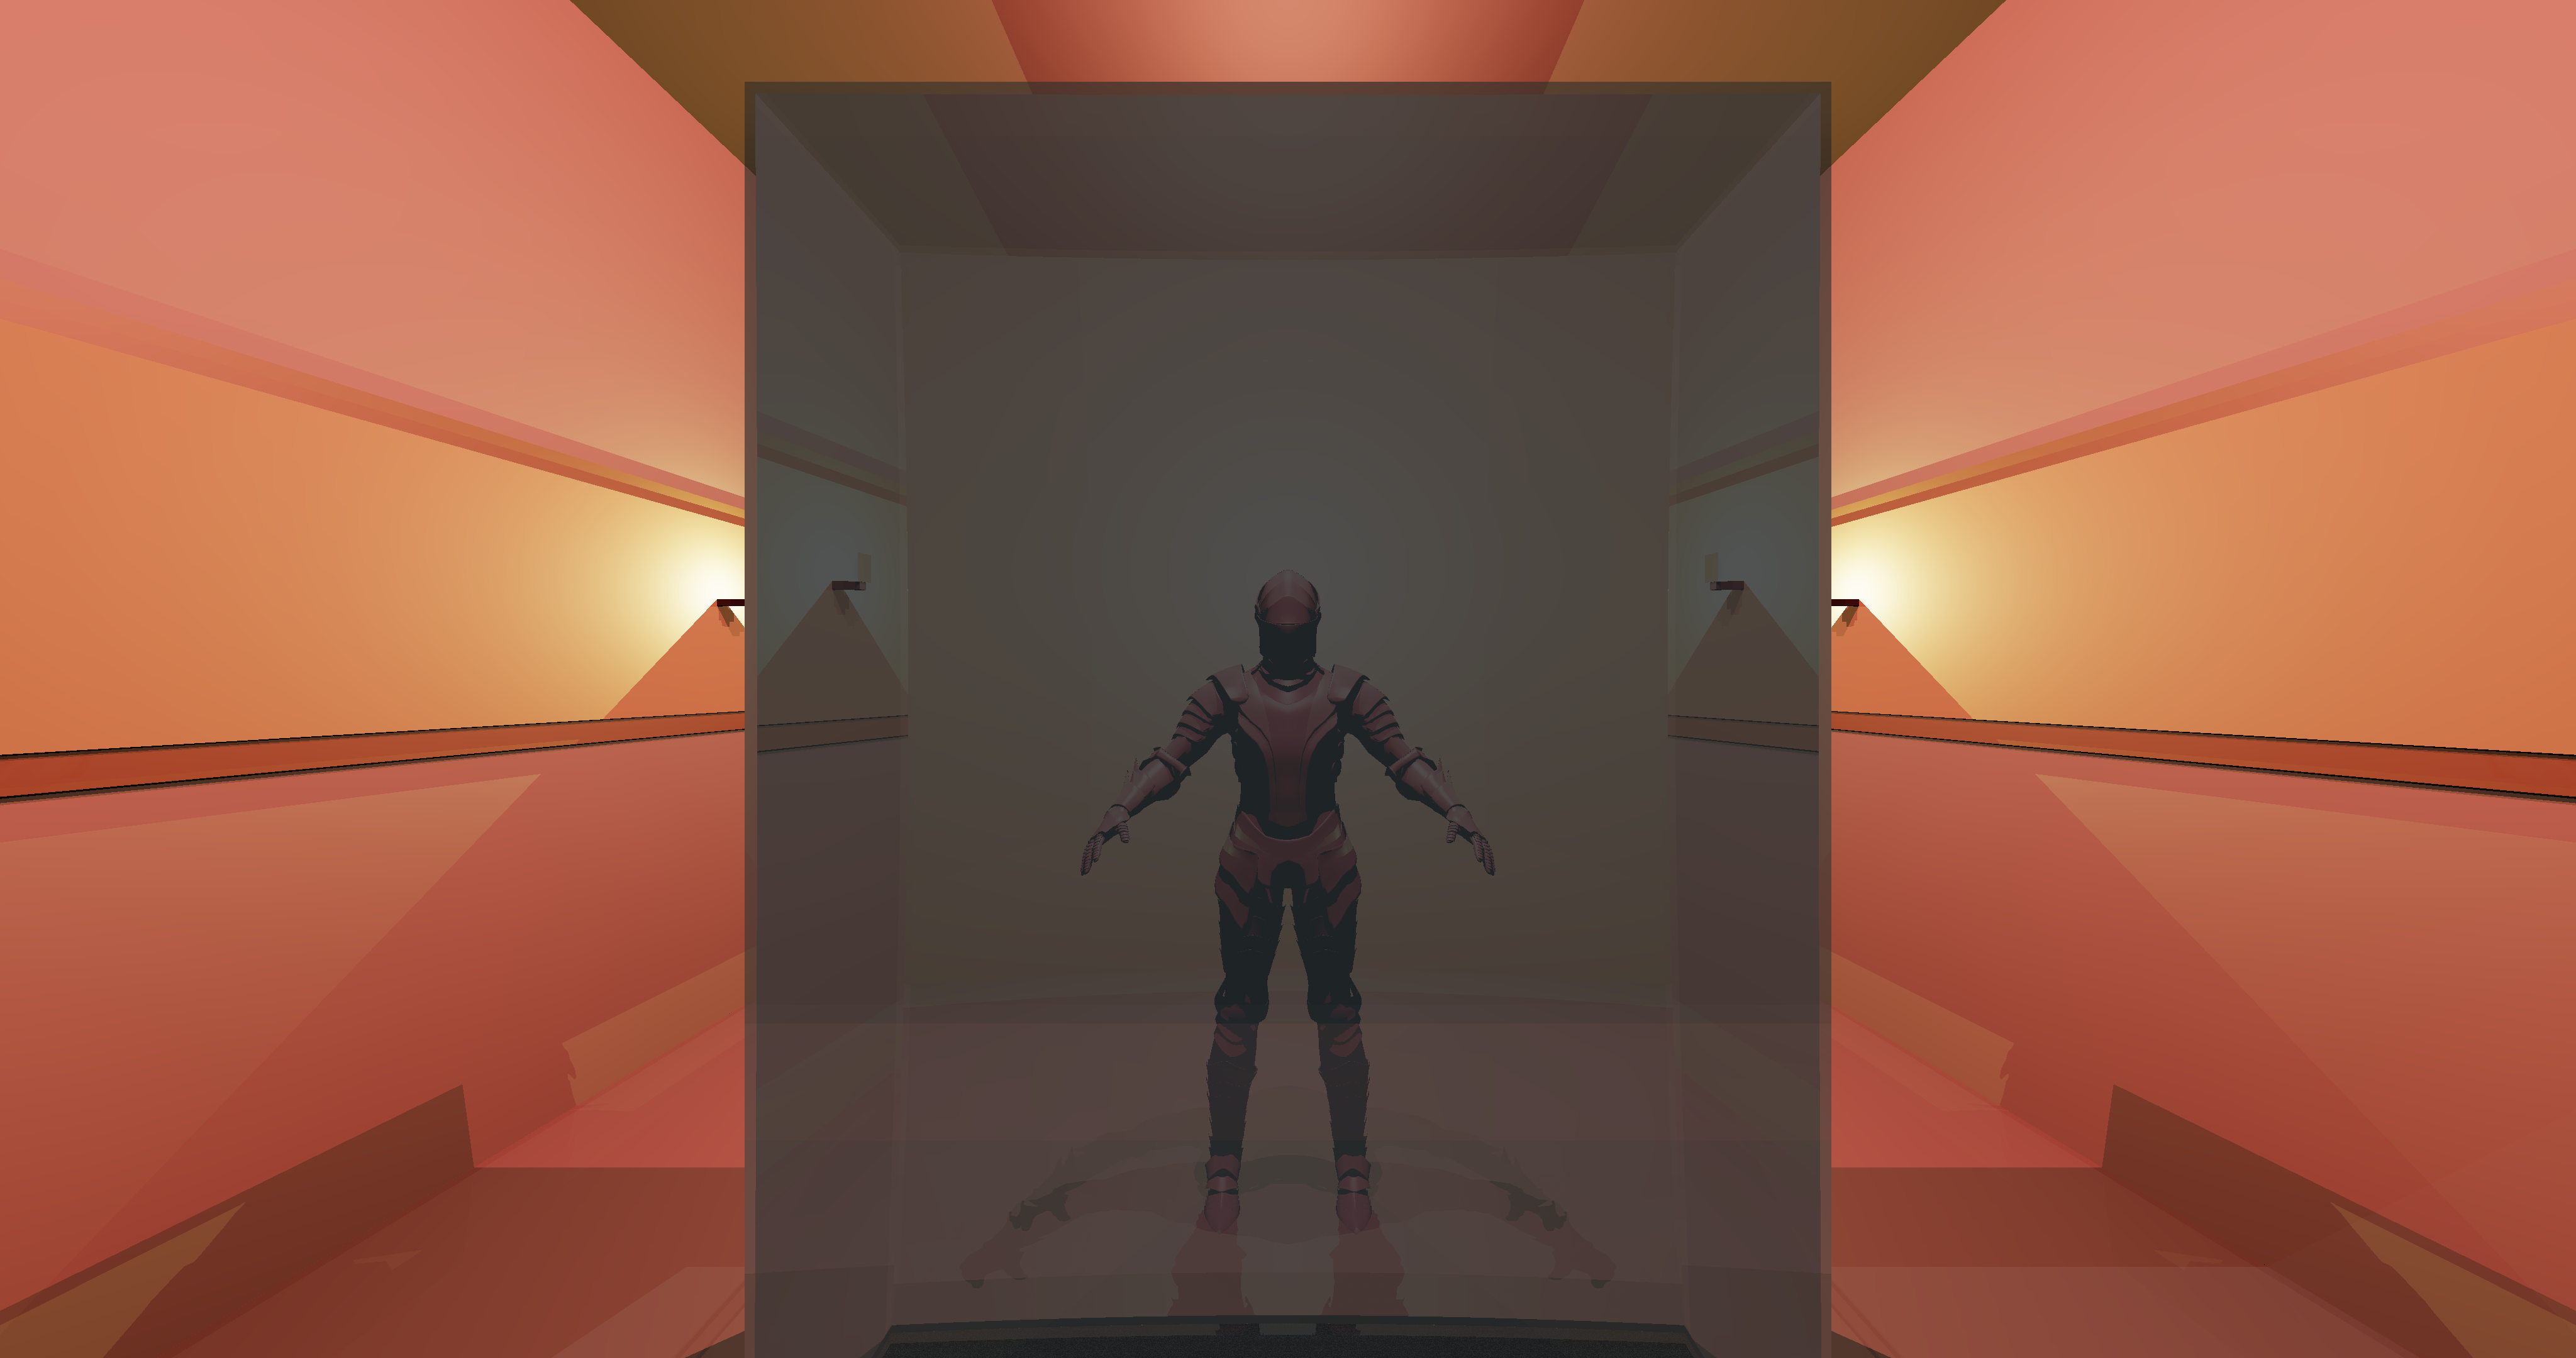
\includegraphics[width=0.7\textwidth]{FrozenGuardian_Test.png}
\caption{Final Render 3: The Frozen Guardian. The ancient guardian is preserved inside a large block of ice.}
\end{figure}

In conclusion, I am very happy with my project because it successfully implements the main requirements of the normal mode. It includes OBJ models, Blinn-Phong materials, multiple light sources, shadows, reflections and refractions. I also added BVH acceleration, and multithreaded rendering to make rendering way faster. I also think I did a very good job inventing stories that went well with the final images.

\end{document}
